\begin{exerciseS}[Linee di corrente, traiettorie e linee di fumo: non stazionario]
 Sia dato il campo di moto
\begin{equation}
 \bm{u}(x,y) = 3 \bm{\hat{x}} + 3t \bm{\hat{y}} 
\end{equation}
Calcolare l'equazione delle linee di corrente, delle traiettorie e delle linee di fumo (curve di emissione) e disegnarle. Infine si determino le tracce generate al tempo $t_0 = 0$ dal segmento che unisce l'origine con il punto $(x_1,y_1)=(0,1)$.
\end{exerciseS}

% \vspace{0.3cm}
\sol

% \vspace{0.3cm}
\partone Definizione di linee di corrente, traiettorie, linee di fumo, tracce. Soluzione di sistemi di equazioni differenziali ordinarie (problemi di Cauchy, ai valori iniziali).

%\begin{itemize}

%\item
%Le linee di corrente sono curve $\bm{S}$ tangenti al campo vettoriale $\bm{u}(\bm{r},t)$ in ogni punto dello spazio $\bm{r}$ e per ogni istante temporale $t$. Essendo curve (1 dimensione), possono essere espresse in forma parametrica, come funzioni di un parametro scalare $p$. La 'traduzione' della definizione in formula è quindi:
%\begin{equation}
% \frac{d\bm{S}(p)}{dp} = \bm{u}(\bm{S}(p),t)
%\end{equation}
%Il vettore tangente ${d\bm{S}(p)}{dp}$ alla curva $\bm{S}(p)$ nel punto ${\bm{S}(p)}$ è parallelo al vettore 
%velocità $\bm{u}$ nello stesso punto $\bm{S(p)}$, al tempo considerato $t$.

%\item
%Le traiettorie descrivono il moto della singola particella fluida e sono descritte dall'equazione:
%\begin{equation}
%\begin{cases}
% \frac{d\bm{R}(t)}{dt} = \bm{u}(\bm{R(t)},t) \\
% \bm{R}(t_0) = \bm{R_0}
%\end{cases}
%\end{equation}
%La traiettoria descritta sopra è quella della particella che all'istante $t_0$ passa per il punto $\bm{R_0}$.
%Interpretazione della formula: la velocità ${d\bm{R}(t)}/{dt}$ della particella (derivata della posizione della
%particella $R(t)$ nel tempo) è uguale alla velocità del fluido nella posizione $R(t)$ nella quale si trova la particella all'istante $t$.

%Fissati $t_0$ e $\bm{R_0}$, si osserva la traiettoria della particella al variare del tempo $t$.

%\item
%Le linee di fumo sono un modo per tracciare tutte le particelle di fluido passate per un determinato punto nello spazio a diversi istanti temporali. La loro equazione è:
%\begin{equation}
%\begin{cases}
% \frac{d\bm{R}(t)}{dt} = \bm{u}(\bm{R},t) \\
% \bm{R}(\tau) = \bm{\bar{R}}
%\end{cases}
%\end{equation}
%L'equazione è identica all'equazione delle traiettorie.
%Cambia la variabile che descrive la curva: si considerano fissi il punto di emissione $\bm{\bar{R}}$ e il tempo
%$t$ al quale viene osservata la curva di emissione; la variabile che descrive la curva di emissione è il tempo
%$\tau$ al quale le particelle passano da $\bm{\bar{R}}$.

%Nel caso di campi stazionari linee di corrente, traiettorie e linee di fumo coincidono.

%\item
%Tracce:
%\begin{equation}
%\begin{cases}
% \frac{d\bm{R}(t)}{dt} = \bm{u}(\bm{R},t) \\
% \bm{R}(\tau) = \bm{\bar{R}}
%\end{cases}
%\end{equation}
%L'equazione è identica all'equazione delle traiettorie e delle curve di emissione.
%Cambia la variabile che descrive la curva: si considerano fissi il tempo $\tau$ e il tempo
%$t$ al quale viene osservata la curva di emissione; la variabile che descrive la curva di emissione è la posizione $\bm{\bar{R}}$ dalle quali passano le particelle.

%\end{itemize}

%\textit{Osservazione}. Non c'è nessuna differenza formale tra $\tau$ e $t_0$ e $\bm{R_0}$ e $\bm{\bar{R}}$.

%\clearpage

% \vspace{0.3cm}
\parttwo
Partendo dalle definizioni, si ricavano le equazioni delle curve caratteristiche. Il problema per le traiettorie, le linee di fumo e le tracce viene risolto una volta sola per ottenere il risultato in forma parametrica in funzione di $t$, $t_0$, $\bm{R_0}(p) = (x_0(p), y_0(p))$. 
\begin{itemize}
\item \textbf{Linee di corrente.} L'equazione vettoriale che definisce una linea di corrente $\bm{S}(p) = X(p) \bm{\hat{x}} + Y(p) \bm{\hat{y}}$ viene scritta per componenti, 
\begin{equation}
 \begin{cases}
  \dfrac{dX}{dp}(p) = \lambda(p) 3 \\
  \dfrac{dY}{dp}(p) = \lambda(p) 3t  \ . \\
 \end{cases}
%  \quad\Rightarrow\quad
%  \frac{dY}{dX} = t
%  \quad\Rightarrow\quad
%  Y = X t + c
\end{equation}
Il sistema di equazioni può essere risolto ricavando dalla prima $\lambda(p)$ in funzione di $dX/dp$, sostituendolo nella seconda, e integrando tra $p_0$ e $p$, con $t$ fissato
% \begin{equation}
%  \dfrac{d Y}{dp}(p) = \dfrac{d X}{dp}(p) t 
% \end{equation}
\begin{equation}
 \int_{p_0}^{p}\dfrac{d Y}{dp}(p') dp' = \int_{p_0}^{p}\dfrac{d X}{dp}(p') \ t \ dp' \quad \rightarrow \quad Y(p) - Y(p_0) = ( X(p) - X(p_0) ) \ t \ . 
\end{equation}
Dopo aver fissato una linea di corrente, imponendo il suo passaggio per un punto, $(X(p_0), Y(p_0)) = (x_0, y_0)$, si ottiene la sua equazione in \textit{forma cartesiana}
\begin{equation}
 y = y_0 + ( x - x_0 ) t \ .
\end{equation}
In questo problema, le linee di corrente costituiscono una famiglia di rette parallele nel piano $x$-$y$, a ogni istante temporale, il cui coefficiente angolare, $t$, aumenta con il tempo.
%
\begin{figure}[h]
\centering
\begin{minipage}{0.30\textwidth}
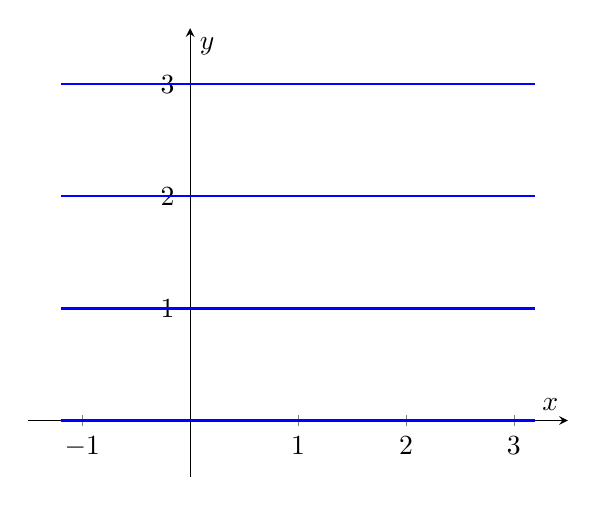
\begin{tikzpicture}
% \begin{axis}[axis lines=middle, domain=-1.2:2.6, xlabel={$x$}, ylabel={$y$} ,
%              xmin = -1.2 , xmax = 2.9, ymin = -0.5 , ymax = 3.2]
\begin{axis}[axis lines=middle, domain=-1.2:3.2, xlabel={$x$}, ylabel={$y$} ,
             xmin = -1.5 , xmax = 3.5, ymin = -0.5 , ymax = 3.5]]
\addplot
[domain=-1.2:3.2,samples=40,smooth,thick,blue]
{0};
\addplot
[domain=-1.2:3.2,samples=40,smooth,thick,blue]
{1};
\addplot
[domain=-1.2:3.2,samples=40,smooth,thick,blue]
{2};
\addplot
[domain=-1.2:3.2,samples=40,smooth,thick,blue]
{3};
%\legend{Linee di corrente a $t=0$}
\end{axis}
\end{tikzpicture}
\end{minipage}\hspace{3.0cm}
\begin{minipage}{0.30\textwidth}
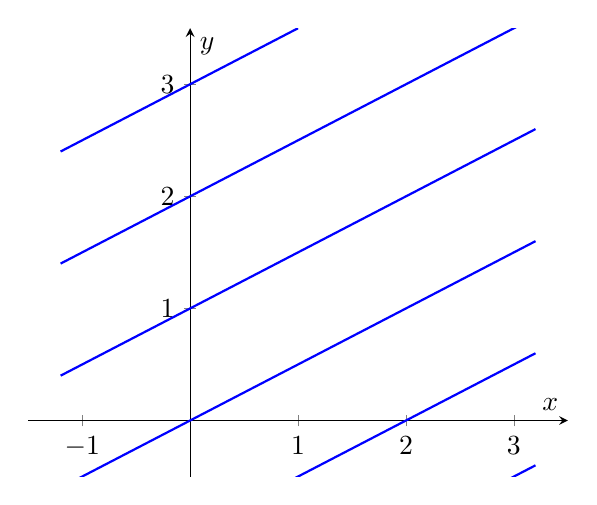
\begin{tikzpicture}
% \begin{axis}[axis lines=middle, domain=-1.2:2.6, xlabel={$x$}, ylabel={$y$} ,
%              xmin = -1.2 , xmax = 2.9, ymin = -0.5 , ymax = 3.2]
\begin{axis}[axis lines=middle, domain=-1.2:3.2, xlabel={$x$}, ylabel={$y$} ,
             xmin = -1.5 , xmax = 3.5, ymin = -0.5 , ymax = 3.5]]
\addplot
[domain=-1.2:3.2,samples=40,smooth,thick,blue]
{0.5*x - 2};
\addplot
[domain=-1.2:3.2,samples=40,smooth,thick,blue]
{0.5*x - 1};
\addplot
[domain=-1.2:3.2,samples=40,smooth,thick,blue]
{0.5*x};
\addplot
[domain=-1.2:3.2,samples=40,smooth,thick,blue]
{0.5*x + 1};
\addplot
[domain=-1.2:3.2,samples=40,smooth,thick,blue]
{0.5*x + 2};
\addplot
[domain=-1.2:1,samples=40,smooth,thick,blue]
{0.5*x + 3};
%\legend{Linee di corrente a $t=0.5$}
\end{axis}
\end{tikzpicture}
\end{minipage}
\caption{Linee di corrente a $t=0.0$ (sinistra) e $t=0.5$ (destra).}
\end{figure}





\item \textbf{Traiettorie.} Le equazioni di traiettorie, linee di fumo e tracce vengono ricavate in forma parametrica risolvendo il problema ai valori iniziali che le definisce. In un secondo momento viene ricavata la loro equazione in \textit{forma cartesiana}, esplicitando il parametro in funzione di una delle due coordinate spaziali, esplicitando il parametro in funzione di una delle due coordinate spaziali. Per le traiettorie, parametrizzate con $t$, si ottiene
\begin{equation}\label{eqn:ese:par}
 \begin{cases}
  \dfrac{dx}{dt}(t) = 3 \\
  \dfrac{dy}{dt}(t) = 3t \\
  x(t_0) = x_0 , \quad y(t_0) = y_0
 \end{cases}
 \quad \rightarrow \quad
 \begin{cases}
  x(t;\bm{R}_0,t_0) = x_0 + 3(t-t_0) \\
  y(t;\bm{R}_0,t_0) = y_0 +\frac{3}{2} (t^2 -t_0^2) \ . \\
 \end{cases}
\end{equation}
Esplicitando $t$ in funzione di $x$, 
\begin{equation}
 t = t_0 + \dfrac{x-x_0}{3} \ ,
\end{equation}
e sostituendo nella coordinata $y$ si ottiene l'equazione in forma cartesiana,
\begin{equation}\label{eqn:ese:trai}
 y(x;\bm{R_0},t_0) = \dfrac{1}{6}x^2 + \left[ -\dfrac{1}{3}x_0 +t_0 \right] x +
 y_0 + \dfrac{1}{6}x_0^2 - x_0 t_0 \ ,
\end{equation}
all'interno della quale $\bm{R}_0 = (x_0,y_0)$ e $t_0$ compaiono ancora come parametri. Dalla (\ref{eqn:ese:trai}), le traiettorie sono parabole con la concavità rivolta verso l'alto.


\begin{figure}[h!]
\centering
\begin{tikzpicture}
\begin{axis}[axis lines=middle, domain=-1.2:3.2, xlabel={$x$}, ylabel={$y$} ,
             xmin = -1.5 , xmax = 3.5, ymin = -1.0 , ymax = 3.5]
\addplot
[domain= 0:3,samples=40,smooth,thick,blue]
{1/6*x^2};
%\legend{Traiettoria per $\bm{R_0}=\bm{0}$, $t_0 = 0$, $t = t_0:1$}
\end{axis}
\end{tikzpicture}
\caption{Traiettoria per $\bm{R_0}=\bm{0} , t_0 = 0 , t \in [0,1]$}
\end{figure}


\item \textbf{Linee di fumo (curve di emissione).} La forma parametrica dell'equazione delle linee di fumo (funzioni di $t_0)$ è
\begin{equation}
 \begin{cases}
  x(t_0;t,\bm{R}_0) = x_0 + 3(t-t_0) \\
  y(t_0;t,\bm{R}_0) = y_0 +\frac{3}{2} (t^2 -t_0^2) \ . \\
 \end{cases}
\end{equation}

Esplicitando $t_0$ in funzione di $x$, 
\begin{equation}
 t_0 = t - \dfrac{x-x_0}{3} \ ,
\end{equation}
e sostituendo nella coordinata $y$ si ottiene l'equazione in forma cartesiana,
\begin{equation}\label{eqn:ese:trai}
 y(x;\bm{R_0},t) = -\dfrac{1}{6}x^2 + \left[ \dfrac{1}{3}x_0 +t \right] x +
 y_0 - \dfrac{1}{6}x_0^2 + x_0 t_0 \ ,
\end{equation}
all'interno della quale $\bm{R}_0 = (x_0,y_0)$ e $t$ compaiono ancora come parametri. Dalla (\ref{eqn:ese:trai}), le linee di fumo sono parabole con la concavità rivolta verso il basso.


\begin{figure}[h!]
\centering
\begin{tikzpicture}
\begin{axis}[axis lines=middle, domain=-1.2:3.2, xlabel={$x$}, ylabel={$y$} ,
             xmin = -1.5 , xmax = 3.5, ymin = -1.0 , ymax = 3.5]]
\addplot
[domain= 0:3,samples=40,smooth,thick,blue]
{-1/6*x^2+x};
%\legend{$\bm{R_0}=\bm{0} , \tau = 0:t , t=1$}
\addplot
[domain= 0:3,samples=40,smooth,dashed,thick,red]
{1/6*x^2};
\addplot
[domain= 0:2.25,samples=40,smooth,dashed,thick,red]
{1/6*x^2+0.25*x};
\addplot
[domain= 0:1.5,samples=40,smooth,dashed,thick,red]
{1/6*x^2+0.50*x};
\addplot
[domain= 0:0.75,samples=40,smooth,dashed,thick,red]
{1/6*x^2+0.75*x};
\end{axis}
\end{tikzpicture}
\caption{Curva di emissione con $\bm{R_0}=\bm{0} , t_0 \in [0,t] , t=1$ (blu) e traiettorie delle particelle passanti per l'origine negli istanti di tempo $t_0=0, 0.25, 0.50, 0.75$, per $t>t_0$ (tratteggiate in rosso).}
\end{figure}

\item \textbf{Tracce.} La forma parametrica dell'equazione delle tracce è
\begin{equation}
 \begin{cases}
  x(\bm{R}_0;t,t_0) = x_0 + 3(t-t_0) \\
  y(\bm{R}_0;t,t_0) = y_0 +\frac{3}{2} (t^2 -t_0^2) \ . \\
 \end{cases}
\end{equation}

Il segmento che unisce l'origine al punto $(x_1,y_1)=(0,1)$ è descritto in forma paramterica come
\begin{equation}
\bm{R_0}(p) = \begin{cases}
 x_0(p) = 0  \\
 y_0(p) = p  \\
\end{cases}  , \quad p \in [0,1] \ .
\end{equation}
La forma parametrica delle tracce ($p$ è il parametro che descrive la curva, mentre $t$, $t_0$ sono parametri fissi) è quindi
\begin{equation}
\bm{R}(\bm{R_0}(p),t,t_0) = 
 \begin{cases}
  x(p;t,t_0) = 3(t-t_0) \\
  y(p;t,t_0) = p +\frac{3}{2} (t^2 -t_0^2) \\
 \end{cases}  , \quad p \in [0,1] \ .
\end{equation}
Queste sono segmenti verticali di lunghezza uguale a 1, con il punto più basso di coordinate $\left(3(t-t_0),\frac{3}{2}(t^2-t_0^2)\right)$.



\begin{figure}[h!]
\centering
\begin{minipage}{0.45\textwidth}
\begin{tikzpicture}
\begin{axis}[axis lines=middle, domain=-1.2:3.2, xlabel={$x$}, ylabel={$y$} ,
             xmin = -1.5 , xmax = 3.5, ymin = -1.0 , ymax = 3.5]]
\addplot[color=blue,mark=x] coordinates{
         (0.0, 0.0)
         (0.0, 1.0)};
\addplot[color=blue,mark=x] coordinates{
         (0.75, 0.656)
         (0.75, 1.656)};
\addplot[color=blue,mark=x] coordinates{
         (1.5, 1.125)
         (1.5, 2.125)};
\addplot[color=blue,mark=x] coordinates{
         (2.25, 1.406)
         (2.25, 2.406)};
\addplot[color=blue,mark=x] coordinates{
         (3.0, 1.5)
         (3.0, 2.5)};
\end{axis}
\end{tikzpicture}
\end{minipage}\hspace{1cm}
\begin{minipage}{0.45\textwidth}
\begin{tikzpicture}
\begin{axis}[axis lines=middle, domain=-1.2:3.2, xlabel={$x$}, ylabel={$y$} ,
             xmin = -1.5 , xmax = 3.5, ymin = -1.0 , ymax = 3.5]]
\addplot[color=red,mark=x,thick] coordinates{
         (0.0, 0.0)
         (0.0, 1.0)};
\addplot[color=red,mark=x,thick] coordinates{
         (0.75, 0.084)
         (0.75, 1.084)};
\addplot[color=red,mark=x,thick] coordinates{
         (1.5, 0.375)
         (1.5, 1.375)};
\addplot[color=red,mark=x,thick] coordinates{
         (2.25, 0.844)
         (2.25, 1.844)};
\addplot[color=red,mark=x,thick] coordinates{
         (3.0, 1.5)
         (3.0, 2.5)};
\end{axis}
\end{tikzpicture}
\end{minipage}
\caption{A sinistra: tracce uscenti dalla curva $\bm{R_0} = (0,p)$, $p \in [0,1]$ agli istanti di tempo $t_0 = 0, 0.25, 0.5, 0.75, 1$ osservate all'istante di tempo $t=1$. A destra: traccia uscente dalla curva $\bm{R_0} = (0,p)$, $p \in [0,1]$ all'istante di tempo $t_0 = 0$, osservata ai tempi $t_0 = 0, 0.25, 0.5, 0.75, 1$}
\end{figure}

% \href{https://www.youtube.com/watch?v=nuQyKGuXJOs}{Collegamento al video del National Committee sulle visualizzazioni.}


\end{itemize}
